\documentclass[tikz]{standalone}

\usetikzlibrary{arrows}

\begin{document}
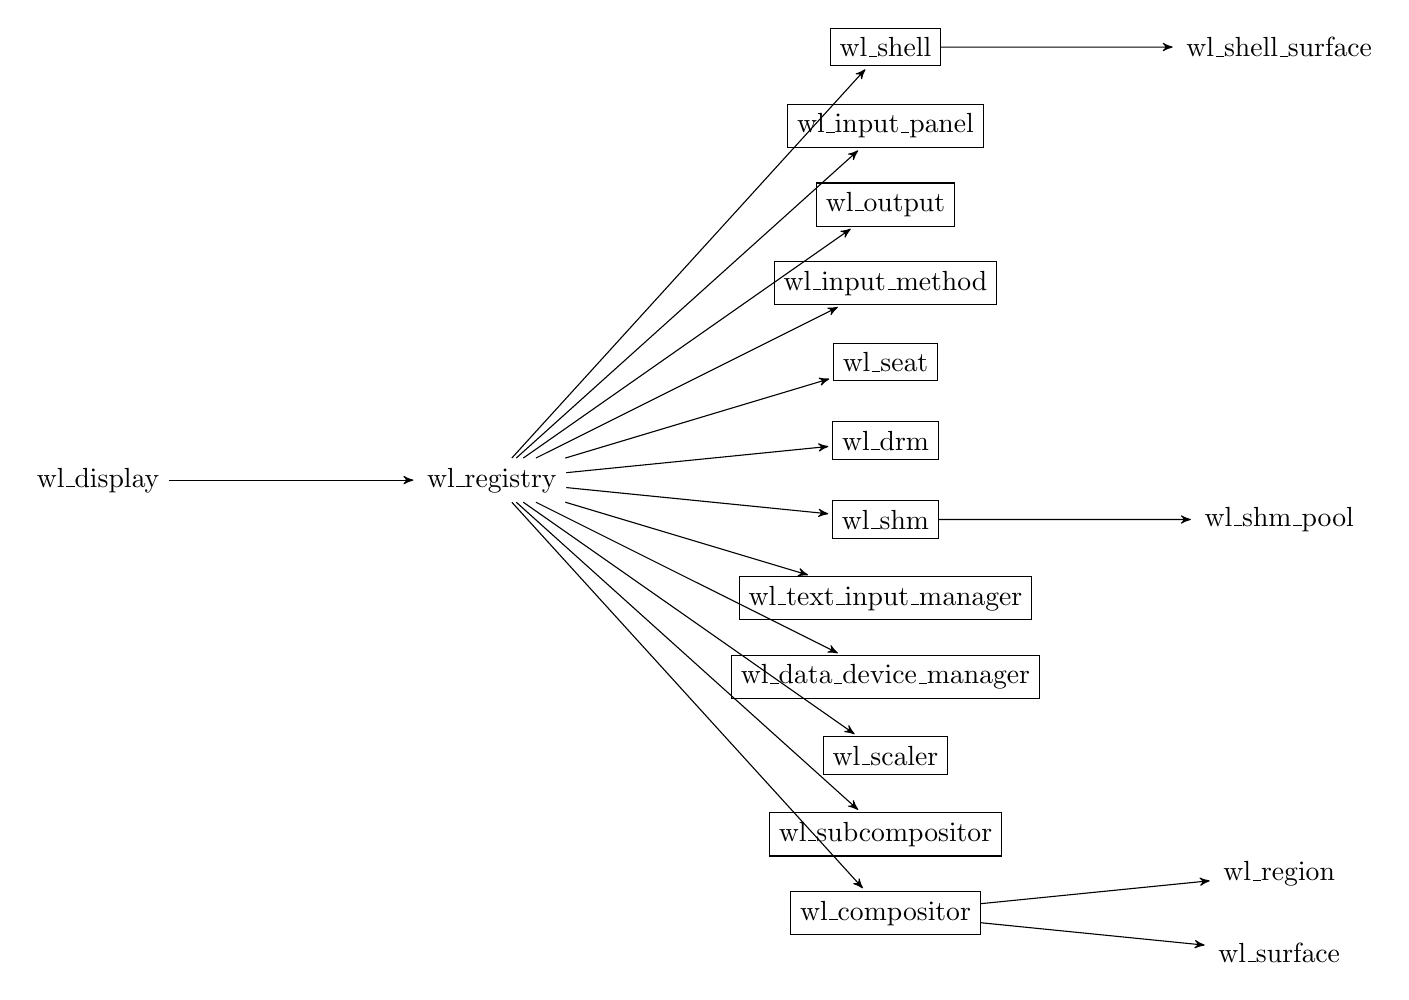
\begin{tikzpicture}[grow=right,->,>=stealth',shorten >=0.5mm, level distance=5cm, sibling distance=1cm]
  \tikzstyle{global} = [draw, rectangle]
  \node {wl\_display}
    child {
      node {wl\_registry}
        child {
          node [global] {wl\_compositor}
            child {
              node {wl\_surface}
            }
            child {
              node {wl\_region}
            }
        }
        child {
          node [global] {wl\_subcompositor}
        }
        child {
          node [global] {wl\_scaler}
        }
        child {
          node [global] {wl\_data\_device\_manager}
        }
        child {
          node [global] {wl\_text\_input\_manager}
        }
        child {
          node [global] {wl\_shm}
            child {
              node {wl\_shm\_pool}
            }
        }
        child {
          node [global] {wl\_drm}
        }
        child {
          node [global] {wl\_seat}
        }
        child {
          node [global] {wl\_input\_method}
        }
        child {
          node [global] {wl\_output}
        }
        child {
          node [global] {wl\_input\_panel}
        }
        child {
          node [global] {wl\_shell}
            child {
              node {wl\_shell\_surface}
            }
        }
    }
  ;
\end{tikzpicture}
\end{document}
